% !TEX root =  fission.tex
%
%
% Use 'make' to run latex and generate the pdf file
%
% Doug Wright
%
% ADC 
%
% COK-2001-600 
% 11-304 Physics concepts such as hydrodynamics, photon transport,
% neutronics, fission, fusion, etc., when no classified information
% or association is revealed.

%\ucrl{UCRL-TM-229496}

\section{User Manual}

This section describes how to use this software library to accurately simulate neutron and gamma-ray emission from individual fission reactions.
The latest version of the library can be downloaded from \httpnuclear. Consult the file \texttt{Release\_notes.txt} in the software release to see the compatibility of this library with specific versions of {\tt MCNPX}, {\tt MCNP6}, and {\tt Geant4}.  Earlier versions of the library are distributed in the public release of {\tt MCNPX 2.7.0}~\cite{MCNPX} and {\tt Geant4}~\cite{Geant1,Geant2}.

The following sections describe how to run this library with {\tt MCNPX}/{\tt MCNP6} (Section~\ref{sec:mcnpx}) and {\tt Geant4} (Section~\ref{sec:geant4}), while Section~\ref{sec:api} describes the programmer's interface. 
For examples of creating a stand-alone executable with the programmer's interface, consult the directory \texttt{regr} in the software release.

\subsection{Limitations of the fission library~\label{Limitations of the fission library}}

The range of neutron energies for which induced fission neutron 
multiplicity data are available in the literature spans the range 
from 0 to 10~MeV, to which corresponds a range of $\bar{\nu}$ 
values.  The sampling of number of neutrons per fission is based on 
either the incident neutron energy or the $\bar{\nu}$ corresponding to 
that energy (depending on the option selected in \textit{setnudist}). 

When sampling is based on $\bar{\nu}$ (the default), 
and the $\bar{\nu}$ is in the range for which we have multiplicity 
data from the literature, that data is used. Outside that 
range, the Terrell approximation is used.

If the user selects the option to sample based on energy, and
the energy is within the range for which we have multiplicity 
data from the literature, that data is used.  If the energy is above 10 MeV, then 
the 10 MeV data is used. As this will be inaccurate as the energy becomes much higher
than 10 MeV, the user should select sampling based on $\bar{\nu}$ in this case. 
The same considerations apply for photofission.

In the case of spontaneous fission, data is only available 
for the following isotopes: $^{232}$Th, $^{232}$U, 
$^{233}$U, $^{234}$U, $^{235}$U, $^{236}$U, $^{238}$U, 
$^{237}$Np, $^{238}$Pu, $^{239}$Pu, $^{240}$Pu, $^{241}$Pu, 
$^{242}$Pu, $^{241}$Am, $^{242}$Cm, $^{244}$Cm, $^{249}$Bk, 
and $^{252}$Cf. 
The Monte-Carlo codes {\tt MCNPX} and {\tt Geant4} do not emit any particles if a different spontaneous fission 
isotope is specified.

% !TEX root =  fission.tex
\pagebreak
\subsection{{\tt MCNPX}}\label{sec:mcnpx}
Version 1.8 of this library was incorporated into the public release of {\tt MCNPX2.7.0}. The authors of this library also maintain private builds of {\tt MCNPX2.7.0} with the most current version of the {\tt LLNL Fission Library}. For users with access to the {\tt MCNPX} source code, upcoming versions of this library can be compiled and linked, see \texttt{src/Recipe\_mcnpx.txt}. Consult the file \texttt{Release\_notes.txt} for comments regarding version compatibility. Currently {\tt MCNPX} provide data cards to activate the fission library (individually for spontaneous, neutron-induced, and photon-induced fission), but do not yet permit changing any of the physics options of the library. 

In addition to adding more neutron multiplicity data and more model options, we made significant modifications to the {\tt MCNPX} treatment of photons, which were then partly carried over into {\tt MCNP6}. The original version of {\tt MCNPX} did not have an analog and discrete treatment for photon emission. Previously photons from fission were included in a total average photonuclear photon count. So it was impossible to have an accurate event-by-event model of photon emission from fission. Our library solved this problem by separating out the photons from the fission process and treating them in a discrete fashion. This took much careful work in cooperation with the {\tt MCNPX} developers. Activating our physics module therefore activates this separate treatment of the fission process as well as provides the features described in this document.

Treatment of fission photons is slightly different in {\tt MCNP6.2}, see {\tt MCNP6.2} User Manual for details.

\subsubsection*{Neutron-induced and spontaneous fission model}

To enable sampling of neutrons and gamma-rays using this fission library set the 6$^{th}$ entry FISM of the PHYS:N card to 5:
\begin{verbatim}
	PHYS:N 5J 5
\end{verbatim}
Note that currently FISM=5 is the only {\tt MCNPX} setting for which gamma-rays are sampled in analog mode for fission reactions. 

Spontaneous fission reactions are activated when definition card SDEF is set to SF:
\begin{verbatim}
	SDEF PAR=SF
\end{verbatim}

In the case of spontaneous fissions, only the isotopes listed in Section~\ref{Limitations of the fission library} have data in the fission library. For other spontaneous fission isotopes, no neutrons, nor gamma-rays are emitted.

\subsubsection*{Photon-induced fission model}

To enable the analog production of photons and neutrons from photofission reactions, the 7$^{th}$ entry FISM of the PHYS:P card should be set to 1:
\begin{verbatim}
        PHYS:P 3J -1 2J 1
\end{verbatim}
When this flag is set, photofission secondaries are sampled only when a photofission event occurs, and are not sampled when other photonuclear reactions occur.

This is different from the default behavior (FISM=0), where photons undergoing photonuclear interactions produce an average number of secondary particles each having a sampled energy/angle though not necessarily from the same photonuclear reaction. The number of secondary particles, as well as their energies and directions are averaged over all possible photonuclear interactions (including photofission). While this default setting is obvisouly not correct microscopically, and we cannot use it to do coincidence counting of photofission neutrons/gammas for instance, it is however correct on average over a large number of interactions.

It is important to note that it is the 4$^{th}$ entry ISPN of the PHYS:P card that controls the analog versus biased nature of the LLNL photofission library collision sampling.

Regarding the data libraries, the physics module needs the ENDF/B-VII photonuclear data library \textit{endf7u}. Lines have to be appended to the file \textit{xsdir} for {\tt MCNPX} to access this photonuclear data library. These lines are also available from the {\tt MCNPX} website. Both \textit{xsdir} and the data library \textit{endf7u} must be in the directory pointed to by the variable DATAPATH.

Photofission is only available for the 39 isotopes listed in Table~\ref{table:photofission isotopes}. Regardless of the option chosen in the $7^{th}$ entry of the PHYS:P card, delayed neutrons and gammas from photofission can be turned on 
and off independently via a different card.

\subsubsection*{Photofission example}

In this example, we will consider a 12 MeV photon beam impinging on a $^{235}$U ball. The photonuclear reaction cross-sections for $^{235}$U are plotted in Fig.~\ref{fig:U-235 photonuclear cross-section}.
%
\begin{figure}[ht]
\begin{center}
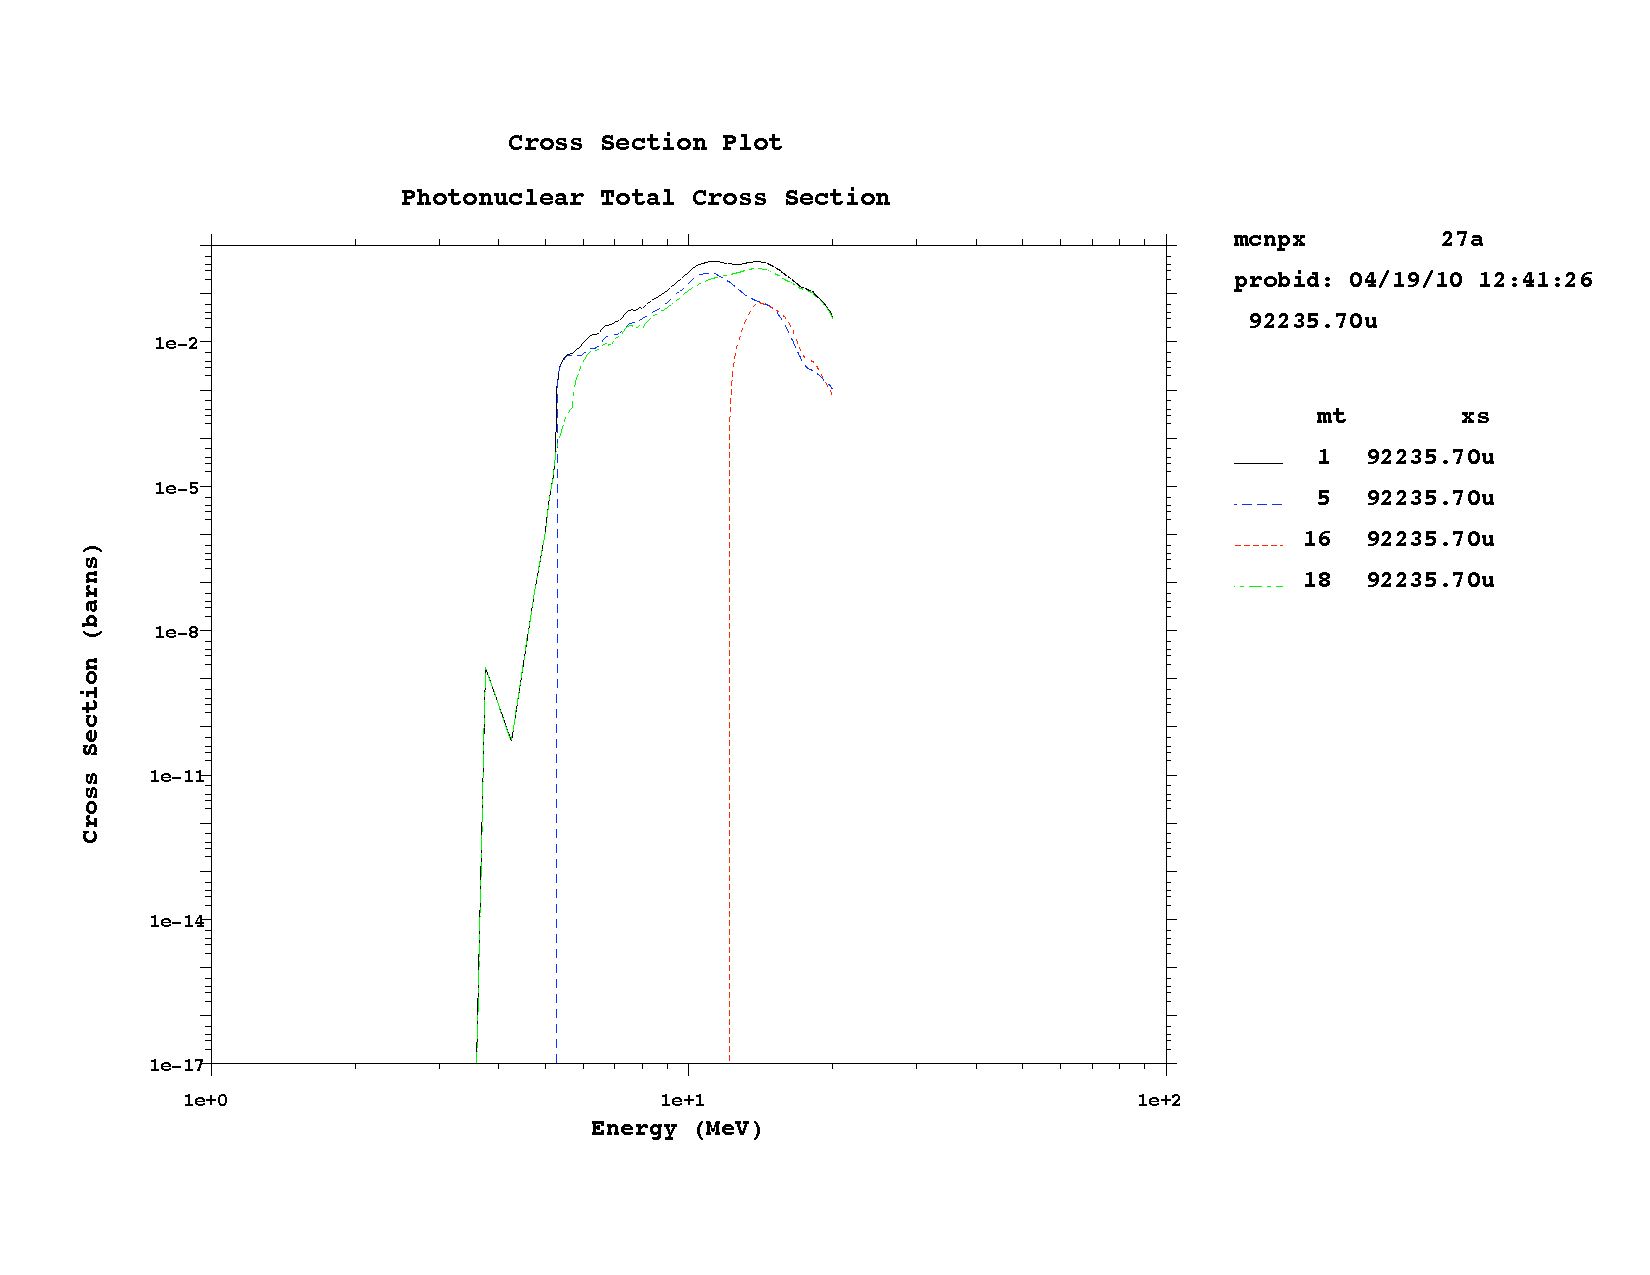
\includegraphics[scale=0.6, angle=0]{eps/92235_photonuclear.pdf}
\end{center}
\caption{Photonuclear cross-sections for $^{235}$U (taken from 92235.70u). Black curve is total, red curve is ($\gamma$,2n), green curve is photofission, blue is all other photonuclear reactions.} 
\label{fig:U-235 photonuclear cross-section}
\end{figure}

The {\tt MCNPX} input deck that describes this example is given below:
{\scriptsize
\begin{verbatim}
12 MeV x-rays into U-235
1 1 -19.0 -1 imp:n=1
2 0 1 imp:n=0

1 so 1.0

mode n p
m1 92235 1 pnlib=.70u
PHYS:P j 1 j -1 2j 1 $ 0=ACE,1=LLNL
sdef par=p erg=12
LCA 7j -2
nps 1000000
f1:n 1
e1 1e-6 199log 12
f11:p 1
e11 1e-3 199log 12
ft11 tag 3
fu11 -1 0.00004 92000.00003 92235.00005 92000.00005 92235.00018 1e10
\end{verbatim}}

To switch from the default ACE {\tt MCNPX} model to the LLNL photofission library, the $7^{th}$ entry of the PHYS:P is set to 1 in the input deck. Note that the $4^{th}$ entry of the PHYS:P card is set to -1 to turn on analog photonuclear particle production. We are interested here in the spectrum of prompt photofission gamma-rays emitted by $^{235}$U. Figure~\ref{fig:energy spectrum of the photofission gamma-rays from a 12 MeV gamma-ray beam impinging on 235U} shows the energy distribution of the photofission gamma-rays for different {\tt MCNPX} settings.

\begin{figure}[ht]
\begin{center}
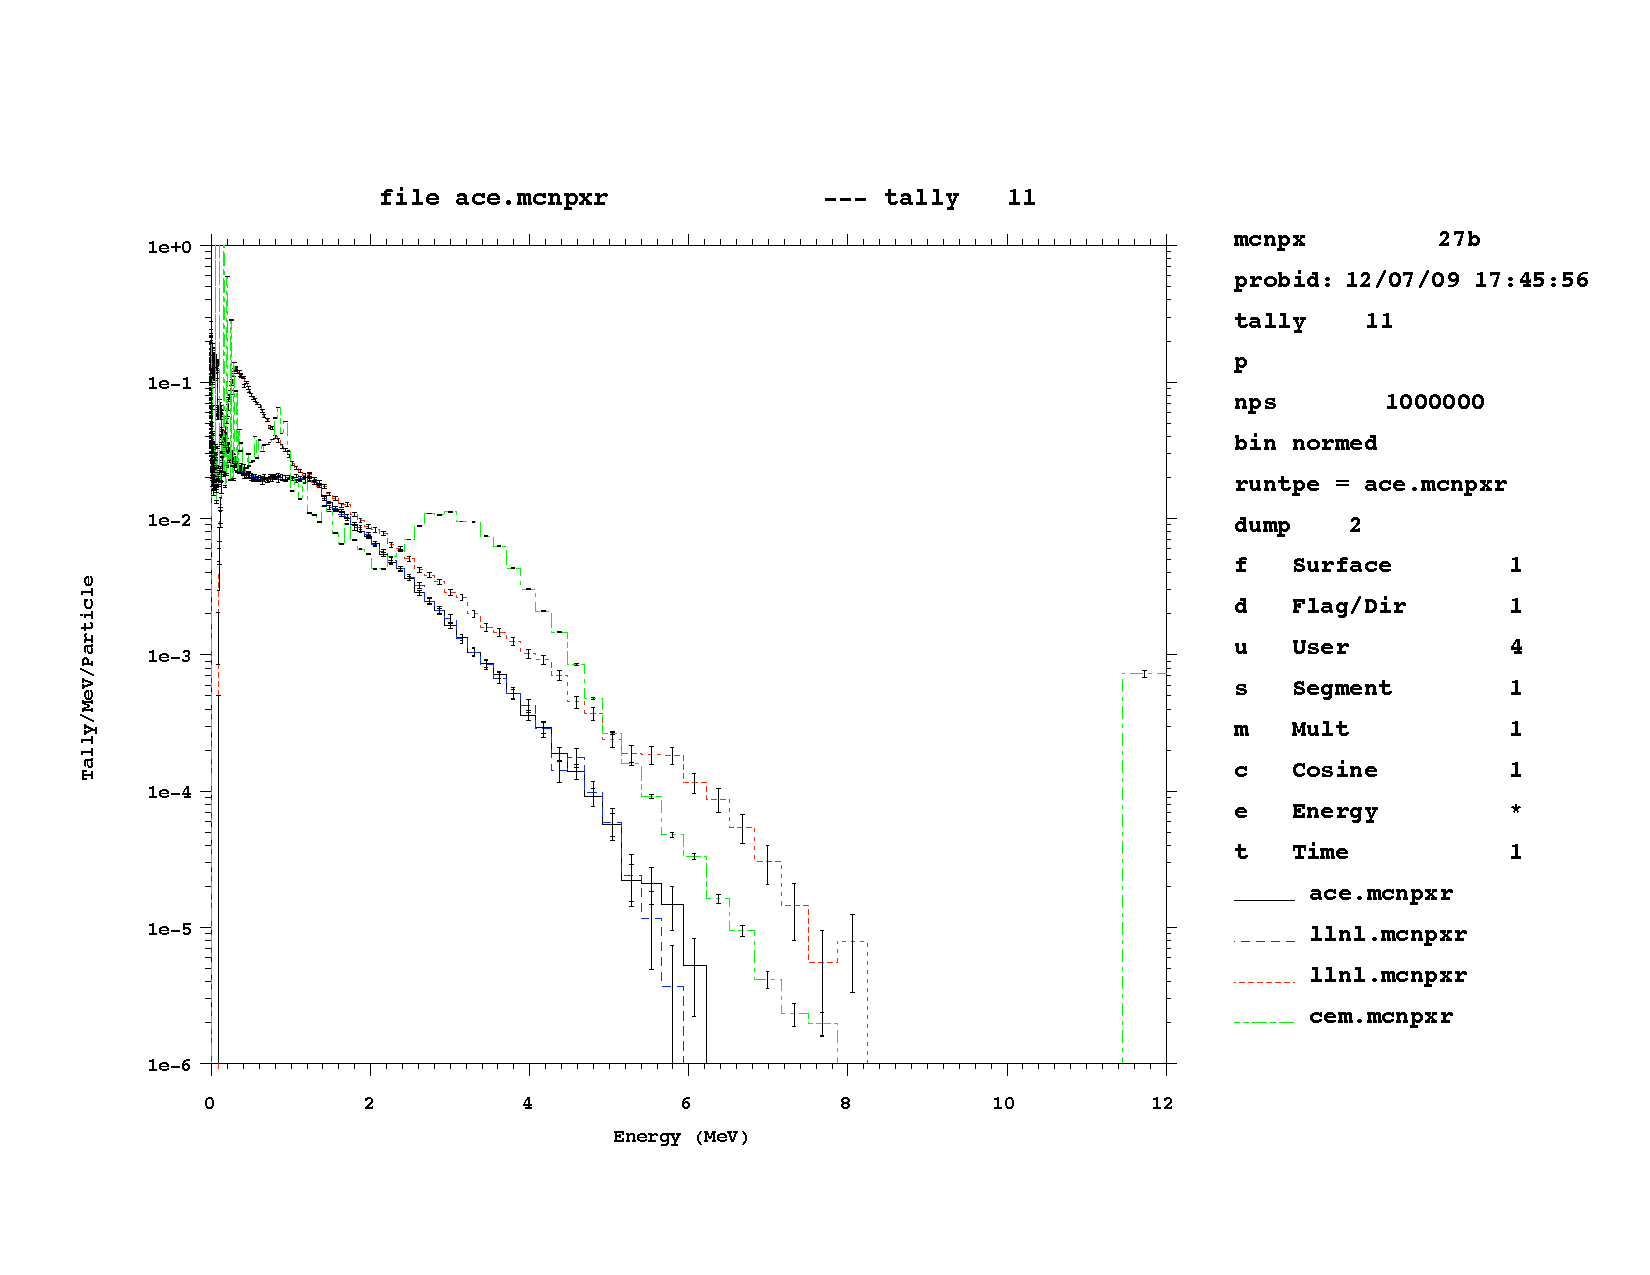
\includegraphics[width=\textwidth]{eps/PhotofissionGammaSpectrum.pdf}
\end{center}
\caption{Energy spectrum of the photofission gamma-rays from a 12 MeV gamma-ray beam impinging on $^{235}$U. The black, blue \& red, and green curves were generated by {\tt MCNPX} simulations with the ACE, LLNL, and CEM models, respectively.}
\label{fig:energy spectrum of the photofission gamma-rays from a 12 MeV gamma-ray
beam impinging on 235U}
\end{figure}

The black curve was generated from a  simulation with the ACE model, it shows the spectrum of all gamma-rays produced 
by photonuclear reactions with the ACE model. The default {\tt MCNPX} ACE model produces prompt photofission 
neutrons but does not produce any prompt photofission gamma-rays, because there is no such data available in the 
photonuclear data libraries ENDF/B-VII. 

The blue and red curves were generated from a simulation where the LLNL photofission library was turned on. The red curve is the spectrum of gamma-rays produced by photofission, while the blue one corresponds to gamma-rays produced by all other photonuclear reactions.

Finally, a last simulation was performed with the much slower CEM model, and the green curve shows the gamma-ray spectrum of all photonuclear reactions with this model.

\subsection{{\tt MCNP6}}\label{sec:mcnp}

Version 1.8 of this library was incorporated into the public release of {\tt MCNP6}. Version 2.0 is now incorporated into {\tt MCNP6.2}. For users with access to the {\tt MCNP6} source code, upcoming versions of this library can be compiled and linked, see \texttt{src/Recipe\_mcnpx.txt}. Consult the file \texttt{Release\_notes.txt} for comments regarding version compatibility.
Currently {\tt MCNP6} provide data cards to activate the fission library (individually for spontaneous, neutron-induced, and photon-induced fission), but do not yet permit changing any of the physics options of the library. 

In {\tt MCNP6.2}, treatment of fission photons is slightly different from what it is in {\tt MCNPX2.7.0}. See {\tt MCNP6.2} User Manual for details.

\subsubsection*{Neutron-induced and spontaneous fission model}

To enable sampling of neutrons and gamma-rays using this fission library set the {\tt METHOD} keyword on the FMULT card
to 5:
\begin{verbatim}
	FMULT zaid METHOD=5
\end{verbatim}
The LLNL fission model is the only way in {\tt MCNP6.2} to produce prompt fission photons. When the LLNL fission multiplicity package is selected (METHOD=5), both the prompt neutrons and the prompt fission photons are fully correlated with the fission event and have multiplicities.

Furthermore, when spontaneous fission reactions are activated, i.e.,
\begin{verbatim}
	SDEF PAR=SF
\end{verbatim}
the LLNL model is the only {\tt MCNP6} method emitting prompt photons for spontaneous fissions. In the case of spontaneous fissions, only the isotopes listed in Section~\ref{Limitations of the fission library} have data in the fission library. For other spontaneous fission isotopes, no neutrons, nor gamma-rays are emitted. Spontaneous fission photons are neglected in the {\tt MCNP6} default FMULT spontaneous fission source.

Delayed fission gammas are independent of the fission model and are controlled by the ACT card.

\subsubsection*{Photon-induced fission model}

When METHOD 5 is selected on the FMULT card and photofission is also turned on (ISPN$\ne$0 and FISM=1 on the PHYS:P card):
\begin{verbatim}
        PHYS:P 3J -1 2J 1
\end{verbatim}
prompt photofission gammas are generated with appropriate photofission neutron correlation and multiplicities. The same remarks as the ones in Sec.~\ref{sec:mcnpx} for the photon-induced fission model, apply here as well.


% !TEX root =  fission.tex
\pagebreak
\subsection{{\tt Geant4}}\label{sec:geant4}

Version 1.2 of this library has been available in the public release of Geant4 since version 4.9.0. 
Geant4.9.6 and later require version 1.9 or later of this library. Version 2.0 of the LLNL Fission Library has been tested with Geant4.10.02 as an external library that overrides the built-in fission library. It is available at \httpnuclear  . 
% To use the built-in version there is no need to download or compile the fission library itself and the standard Geant4 makefile is sufficient. 
An example of building a Geant4 executable and activating the fission library is given in the \texttt{geant} directory 
in the fission library source code distribution. This directory also includes an example and explicit instructions for overriding the built-in fission library with the latest version.

\subsection*{Limitations}

The neutron-induced fission data available in G4NDL4.5 is limited. At the time of this writing, there are only data files for  isotopes of radium, actinium, thorium, protactinium and uranium. The origin of the data has not been investigated. For other isotopes, induced fission will not emit any particles. This fission library does not have any spontaneous fission data for isotopes other than the ones listed in section~\ref{Limitations of the fission library}.
Photofission has not been implemented in {\tt Geant4}.

\subsection*{Execution}

The environment variable \textit{NeutronHPCrossSections} must point to the G4NDL directory, where the induced fission cross-sections and data are located.

\subsection*{Description of the C++ classes}


For neutron induced fission, this model is intended to be used with
the low energy neutron interaction data libraries with class
\textit{G4Fisslib} specified in the physics list as the
\textit{G4HadronFissionProccess} instead of class
\textit{G4NeutronHPFission}.\notgeant{
Here is an example code snippet for registering this model in the physics 
list: \begin{verbatim}
    G4ProcessManager* pmanager = particle->GetProcessManager();
    G4String particleName = particle->GetParticleName();

    if (particleName == "gamma") {
      (...)
    } else if (particleName == "neutron") {
      (...)
      // Fission library model
      G4HadronFissionProcess *theFissionProcess = new G4HadronFissionProcess();
      G4FissLib* theFissionModel = new G4FissLib;
      theFissionProcess->RegisterMe(theFissionModel);
      pmanager->AddDiscreteProcess(theFissionProcess);
      (...)
    } else ...
\end{verbatim}
}
The constructor of \textit{G4FissLib}
does two things. First it reads the necessary fission cross-section
data in the file located in the directory specified by the environment
variable \textit{NeutronHPCrossSections}. It does this by initializing
one object of class \textit{G4NeutronHPChannel} per isotope present in
the geometry. Second, it registers an instance of
\textit{G4FissionLibrary} for each isotope as the model for that
reaction/channel. When Geant4 tracks a neutron to a reaction site and
the fission library process is selected among all other process for
neutron reactions, the method \textit{G4FissLib::ApplyYourself} is
called, and one of the fissionable isotopes present at the reaction
site is selected. This method in turn calls
\textit{G4NeutronHPChannel::ApplyYourself} which calls
\textit{G4FissionLibrary::ApplyYourself}, where the induced neutrons
and gamma-rays are emitted by sampling the fission library.

For spontaneous fission the user must provide classes {\it
PrimaryGeneratorAction}, {\it MultipleSource}, {\it
MultipleSourceMessenger}, {\it SingleSource}, {\it SponFissIsotope} to
generate spontaneous fission neutrons and gammas. Examples of these
classes can be downloaded from \httpnuclear. Spontaneous fissions are
generated in the {\it PrimaryGeneratorAction} class.
The spontaneous fission
source needs to be described in terms of geometry, isotopic
composition and fission strength. Once this information is given, the
constructor creates as many spontaneous fission isotopes of class {\it
SponFissIsotope} as specified, and adds them to the source of class
{\it MultipleSource}. When Geant needs to generate particles, it calls
the method {\it PrimaryGeneratorAction::GeneratePrimaries}, which
first sets the time of the next fission based on the fission rates
entered in the constructor, and then calls the method {\it
MultipleSource::GeneratePrimaryVertex} which determines which one of
the spontaneous fission isotopes will fission. This method in turn
calls the method {\it SponFissIsotope::GeneratePrimaryVertex} for the
chosen isotope. It is in this method that the neutrons and photons
sampled from the fission library are added to the stack of secondary
particles.  Sources other than spontaneous fission isotopes can be
added to the source of class {\it MultipleSource}. For instance, a
background term emitting a large number of background gamma-rays can
be added, as long as it derives from the class {\it SingleSource}. The
intensity of that source would be set the same way as for the
spontaneous fission isotope sources.



%\pagebreak
\subsection{COG}
This physics module has been submitted to the COG development team
and will appear in a future release.  The fission library libFission.a
can be sampled for induced fissions in COG using the \textit{FISSLIB}
keyword in the MIX block of the input deck. This is not the
default. The \textit{NUOPTION} can not be used concurrently, it is not
compatible with \textit{FISSLIB}.

COG is similar to MCNPX in that it emits a number of gamma-rays
at each neutron collision site, and this number is independent
on the reaction type. The keyword \textit{NOGAMPRO} can be used
to completely turn off this gamma-ray production.

Spontaneous fissions are implemented using a COG user source.
A sample user source {\tt spfiss.F} is available in the COG distribution 
subdirectory {\tt usrsor}. Compiling a COG user source is easy:
\begin{verbatim}
	make -f COGUserlib.make in=spfiss.F
\end{verbatim}
Using the right compiler at compile time is important, and if this
becomes an issue, a COG developer should be contacted. It is also 
important to use a COG version that is compatible with user
sources and user detectors. Not all COG versions work with
user sources/detectors. Photofission has not been implemented in
COG.

An example of input deck using the {\tt spfiss.F} spontaneous
fission source is located in the {\tt usrsor} directory. The important
lines related to the user source are in the SOURCE block:

{ \small
\begin{verbatim}
SOURCE
NPART = 5e4  $ NPART is the sum of spontaneous fission neutrons and photons
$ 
$ The source below is for a HEU shell (93% enriched in U-235).
$ We neglect here the spontaneous fissions in U-235. The fission rate 
$ for 350 g of U-238 is 350[g]*1.36*10E-2[n/g/s] = 4.76 n/s. With
$ spontaneous nubar equal to 2.01, we have 
$  4.76[n/s]/2.01[n/fission] = 2.368 fissions/sec
$      name    isotope  strength  xcenter  ycenter  zcenter  Rin  Rout  FissRate
$              (1)      (2)       (3)      (4)      (5)      (6)  (7)   (8)
USRSOR spfiss  92238    1.        0.       0.       0.       1.   3.96  2.368
$
\end{verbatim}
}
NPART is the sum of all source particles, that is both spontaneous
fission neutrons and gamma-rays. The line USRSOR has several arguments:
The argument under {\tt name} specify the FORTRAN subroutine to be used a 
the spontaneous fission source: {\tt spfiss}. The first numeric argument is 
the isotope in the form ZA, followed by the source strength (not relevant
in this case), the center of the shell (x, y, z), the inner and outer
radii and the fission rate in fissions/second. Note the units of the
fission rate, fissions/second and not neutrons/second.


% !TEX root =  fission.tex
\pagebreak
\subsection{Fission library interface}\label{sec:api}

The interface to the fission library consists of 27 C functions, each of which will be described below. For examples of creating a stand-alone executable with the programmer's interface, consult the directory \texttt{regr} in the software release.

\subsection*{void genspfissevt\_(int *isotope, double *time)}
This function is called to trigger a spontaneous fission. Multiple neutrons and gamma-rays are generated and stored in a stack along with their energies, directions and emission times. The arguments of this function are

\begin{tabbing}
\indent isotope: \=entered in the form ZA (e.g. 94239 for $^{239}$Pu) \\
\indent time: \> the time of the spontaneous fission \\
\end{tabbing}

The generated neutrons and gamma-rays, along with their properties will be lost upon the next call to genspfissevt\_(),
genfissevt\_() or genphotofissevt\_(). Therefore, they must be retrieved immediately by the caller using the appropriate 
functions described below.

\subsection*{void genfissevtdir\_(int *isotope, double *time, double *nubar, double *eng, double *ndir)}
This function is called to trigger a neutron-induced fission. In addition to the arguments above, the fission inducing neutron
is characterized by:

\begin{tabbing}
\indent nubar: \= user-specified average number of neutrons emitted per fission (e.g. as tabulated in the \\ 
\> cross-section libraries used by the particle transport code) \\
\indent eng: \> energy of the neutron inducing fission \\
\indent ndir: \> normalized incident neutron direction, array with three elements (u,v,w) \\
\end{tabbing}

Either the average number $\bar{\nu}$ of neutrons emitted per fission or the energy \textit{eng} of the fission inducing 
neutron will be used to determine the number of neutrons sampled, see function setnudist\_ below. The number 
of gamma-rays sampled only depends on $\bar{\nu}$. Similarly to genspfissevt\_(), the generated neutrons and gamma-rays are lost upon subsequent calls to genspfissevt\_(), genfissevt\_() or genphotofissevt\_(). The direction $ndir$ of the incident neutron is only used by the {\tt FREYA} model.

\subsection*{void genfissevt\_(int *isotope, double *time, double *nubar, double *eng)}
Same as call to {\bf genfissevtdir\_()} but {\tt FREYA} samples the incident neutron direction randomly.

\subsection*{void genphotofissevt\_(int *isotope, double *time, double *nubar, double *eng)}
This function is called to trigger a photon-induced fission. In addition to the arguments specified in genfissevt\_, the 
fission inducing neutron is characterized by:

\begin{tabbing}
\indent nubar: \= user-specified average number of neutrons emitted per photofission (e.g. as tabulated in the \\ 
\> photonuclear cross-section libraries used by the particle transport code) \\
\indent eng: \> energy of the photon inducing fission \\
\end{tabbing}

Either the average number $\bar{\nu}$ of neutrons emitted per photofission or the energy \textit{eng} of the fission inducing 
photon will be used to determine the number of neutrons sampled, see function setnudist\_ below. The number of gamma-rays sampled only depends on $\bar{\nu}$. Similarly to genspfissevt\_(), the generated neutrons and gamma-rays are lost upon subsequent calls to genspfissevt\_(), genfissevt\_() or genphotofissevt\_().

\subsection*{int getnnu\_() and int getpnu\_()}

These functions return the numbers of fission neutrons and gamma-rays emitted in the fission reaction, or -1 if no number could be sampled in the fission library due to lack of data. The reader is referred to the physics reference manual to find the list of isotopes for which sampling will return positive numbers.

\subsection*{double getneng\_(int *index) and 
double getpeng\_(int *index) \newline
double getnvel\_(int *index) and 
double getpvel\_(int *index)}

These functions return the energies and velocities of the neutrons/gamma-rays.

\subsection*{double getndircosu\_(int *index), double getndircosv\_(int *index), \newline double getndircosw\_(int *index) \newline \newline
double getpdircosu\_(int *index), double getpdircosv\_(int *index), \newline double getpdircosw\_(int *index)}

These 2 families of functions return the direction cosines of the velocity vector on the x, y and z axes for the fission 
neutrons and gamma-rays.

\subsection*{double getnage\_(int *index) and double 
getpage\_(int *index)}

This functions returns the age of the fission neutron/gamma-ray, or -1 if index is out of range. The age returned might be 
different from the time specified in genfissevt\_(), genspfissevt\_() and genphotofissevt\_() for delayed neutrons and gamma-rays, see function setdelay\_() below. Currently, delayed fission neutrons/gamma-rays are not implemented, so all fission products 
are emitted promptly.

\subsection*{void setdelay\_(int *delay)}~\label{setdelay}

This function is called to enable delayed neutrons and gamma-rays. The argument \textit{delay} is set to 

\begin{tabbing}
\indent0 (default) \= for strictly prompt neutrons and photons \\
\indent1 (n/a) \> for prompt neutrons, prompt and delayed photons \\
\indent2 (n/a) \> for prompt and delayed neutrons, prompt photons \\
\indent3 (n/a) \> for prompt and delayed neutrons, prompt and delayed photons \\
\end{tabbing}

Delayed neutrons and gamma-rays have not yet been implemented in the fission library. This setting has presently no effect on the age sampling. All neutrons and photons are currently emitted promptly (delay=0).

\subsection*{void setcorrel\_(int *correlation)}\label{setcorrel}

This function is called to set the type of neutron/gamma-ray correlation.  The argument \textit{correlation} is set to

\begin{tabbing}
\indent 0 (default) \= for no correlation between neutrons and photons \\
\indent 1 \> \parbox[t]{5.5in}{total fission neutron energy and total fission gamma-ray energy are sampled from normal distributions of means given in Beck et al.~\cite{Beck 2007}. No correlation between the number of neutrons and the number of gamma-rays} \\
\indent 2 \> \parbox[t]{5.5in}{total fission neutron energy and total fission gamma-ray energy are sampled from normal distributions of means given in Vogt~\cite{Vogt 2008}. No correlation between the number of neutrons and the number of gamma-rays} \\
\indent 3 \> \parbox[t]{5.5in}{number and energy correlation between neutrons and photons provided by {\tt FREYA} whenever available.} \\
\end{tabbing}

% !TEX root =  fission.tex
\subsection*{void setnudist\_(int *nudist)
\label{setnudist}}

This selects the data to be sampled for the neutron number distributions for neutron-induced fission. If there is no data
available, then in all cases the Terrell approximation is used. The argument \textit{nudist} can take 3 values:

\begin{tabbing}

\indent 0 \hspace*{.55in} \= \parbox[t]{5.5in}{ Use the fit to the Zucker and Holden tabulated P$_\nu$ distributions as a function of energy for $^{235}$U, $^{238}$U and $^{239}$Pu.}\\

\indent 1 \> \parbox[t]{5.5in}{Use fits to the Zucker and Holden tabulated P$_\nu$  distribution as a function of energy for $^{238}$U and  $^{239}$Pu, and a fit to the Zucker and Holden data as well as the Gwin, Spencer and Ingle data (at thermal 
 energies) as a function of energy for $^{235}$U.}\\

\indent 2 \> \parbox[t]{5.5in}{Use the fit to the Zucker and Holden tabulated P$_\nu$ distributions as a function of $\bar{\nu}$. The $^{238}$U fit is used for the $^{232}$U, $^{234}$U, $^{236}$U and $^{238}$U isotopes, the $^{235}$U fit for $^{233}$U 
and $^{235}$U, the $^{239}$Pu fit for $^{239}$Pu and $^{241}$Pu.}\\

\indent 3 (default) \> \parbox[t]{5.5in}{Use the discrete Zucker and Holden tabulated P$_\nu$ distributions and corresponding $\bar{\nu}$s. Sampling based on the incident neutron $\bar{\nu}$. The $^{238}$U data tables are used for the $^{232}$U, $^{234}$U, $^{236}$U  and $^{238}$U isotopes, the $^{235}$U data for $^{233}$U and $^{235}$U, the $^{239}$Pu data for $^{239}$Pu and $^{241}$Pu.}

\end{tabbing}

\subsection*{void setcf252\_(int *ndist, int *neng)}

This function is specific to the spontaneous fission of $^{252}$Cf. It selects the data to be sampled for the neutron number and energy distributions and takes the following arguments:

\begin{tabbing}
\indent ndist: \= Sample the number of neutrons \\
\indent \> 0 (default) \= 
from the tabulated data measured by Spencer \\
\indent \> 1 \> from 
Boldeman's data \\
\\
\indent neng: Sample the spontaneous fission 
neutron energy \\
\indent \> 0 (default)\> from Mannhart corrected  Maxwellian spectrum \\
\indent \> 1 \> from Madland-Nix theoretical spectrum \\
\indent \> 2 \> from the Froehner Watt spectrum \\
\end{tabbing}

\subsection*{void getfreya\_errors\_(int *length, char *error)}
When called, this function returns potential errors that could have occurred in {\tt FREYA}; for instance if the data required by {\tt FREYA} cannot be found. It takes the following arguments:
\begin{tabbing}
\indent length: \= length of error message \\
\indent error: \> pointer to an allocated array of characters devoted to the error message \\
\end{tabbing}
When returning, the length of the error message will be 1 is no error occurred. It will be greater than 1 otherwise.

\subsection*{void setfreyadatapath\_(char *path)}
This function is called to set the path to the directory where the data required by {\tt FREYA} is located. It takes the following argument:
\begin{tabbing}
\indent path: \= character string containing the path to the directory containing the data required by {\tt FREYA}. \\
\end{tabbing}



\subsection*{void setrngf\_(float (*funcptr) (void)) and void setrngd\_(double (*funcptr) (void))}

This function sets the random number generator to the user-defined
one specified in the argument. If either setrngf\_() or setrngd\_() are
not specified, the default system call srand48() is used. The 
arguments are random number generator functions that returns 
variables of type float and double respectively.

